% TEMPLATE for Usenix papers, specifically to meet requirements of
%  USENIX '05
% originally a template for producing IEEE-format articles using LaTeX.
%   written by Matthew Ward, CS Department, Worcester Polytechnic Institute.
% adapted by David Beazley for his excellent SWIG paper in Proceedings,
%   Tcl 96
% turned into a smartass generic template by De Clarke, with thanks to
%   both the above pioneers
% use at your own risk.  Complaints to /dev/null.
% make it two column with no page numbering, default is 10 point

% Munged by Fred Douglis <douglis@research.att.com> 10/97 to separate
% the .sty file from the LaTeX source template, so that people can
% more easily include the .sty file into an existing document.  Also
% changed to more closely follow the style guidelines as represented
% by the Word sample file. 

% Note that since 2010, USENIX does not require endnotes. If you want
% foot of page notes, don't include the endnotes package in the 
% usepackage command, below.

\documentclass[letterpaper,twocolumn,10pt]{article}
\usepackage{usenix,epsfig,endnotes}

\usepackage{amsmath}
\usepackage{amssymb}
\usepackage{float}
\usepackage{mathtools}
\usepackage{marginnote}
\usepackage[outline]{contour}
\usepackage{MnSymbol}
\usepackage{stmaryrd}
\usepackage{cancel}
\usepackage{xcolor}

\begin{document}

%don't want date printed
\date{December 11, 2024}

%make title bold and 14 pt font (Latex default is non-bold, 16 pt)
\title{\Large \bf COS597E Project Final Report: \href{https://github.com/mw6136/NGA\_LeWI}{\texttt{NGA\_LeWI}} \\ Dynamic Load Balancing in a Massively Parallel Reacting Flow Solver}

\author{
{\rm Michael D. Walker \footnotemark
}\\
Princeton University
}

\maketitle 

% Use the following at camera-ready time to suppress page numbers.
% Comment it out when you first submit the paper for review.
% \thispagestyle{empty}

\addtocounter{footnote}{1}
\footnotetext{netID: \texttt{mw6136}\\
Email: \url{michael.walker@princeton.edu}\\
Computational Turbulent Reacting Flow Laboratory (\href{https://ctrfl.princeton.edu/}{CTRFL}) \\
Department of Mechanical and Aerospace Engineering \\ Princeton University, Princeton, NJ 08544 \\
Submitted: December 11, 2024 for fulfillment of  \\
COS597E: Programming Languages, Distributed Systems}

\subsection*{Abstract}
Chemically-reacting flows, like combustion, are highly non-linear. Reaction kinetics follow an exponential Arrhenius law. Such a flow is simulated by applying the system of conservative partial differential equations over a domain, often with a finite-difference discretization and parallelized across many processing units. Using the operator-splitting technique commonly applied in reactive flow solvers, chemistry can be treated as an independent stiff ordinary differential equation (ODE) system within each computational cell, but large variation in the convergence rates of the ODE integrator may occur. Calculation of the chemical source terms in the system of equations, therefore, can lead to severe load imbalance across a distributed computing architecture. The independent nature of the chemistry ODE system leads to a problem that can be parallelized and balanced during the flow solution without the introduction of significant error. This work implements Lend When Idle (LeWI), a program that monitors and dynamically balances the load distribution across cores, on an existing massively parallel reacting flow solver, \texttt{NGA}, providing significant speed-up in clock time. Additionally, a reference mapping scheme is developed which applies reference variables, like mixture fraction $Z_i$ and activation temperature $T_i$, to predict areas of low chemical reaction activity (and thus low computational load). Rather than evaluating the full chemical Jacobian in these regions, a reference cell solution is simply copied, thereby generating further speed-up. Performance is evaluated by comparing to simulations of hydrogen-air and methane-air jet flames, whose unbalanced results were published previously \cite{LACEY2021,Lacey_thesis}. A modest improvement is shown, especially for early simulation timesteps, where computational load is most difficult to predict.

\section{Introduction and Motivation}

Modern Computational Fluid Dynamics (CFD) software relies on distributed-memory parallel computer architectures for large-scale computations. Using resources efficiently while at the same time maintaining high accuracy of the numerical solution is a major challenge. \emph{Computational load imbalance} is a well-known performance issue in multiprocessor reacting flow (e.g., combustion) simulations utilizing directly integrated chemical kinetics. As the need for more detailed combustion models has become prominent, chemical kinetics models have grown in size and complexity, resulting in higher computational cost and often exceeding the computational cost of fluid dynamics by a factor of 100 \cite{Law_book}. 

For each chemical reaction $j$ with species $\mathcal{A}_k$ (such as oxidizer and fuel) and stoichiometric coefficients $\nu_k$: 
$$\nu^f_{k,j} \mathcal{A}_k \leftrightarrow \nu^b_{k,j} \mathcal{A}_k \quad ,$$
where $f$ and $b$ scripts indicate the forward and backward modes of an equilibrium reaction. The governing reaction rate $\dot{\omega}_j$ is defined by
$$\dot{\omega}_j = k_{f,j} \prod^k (\frac{\rho Y_k}{W_k})^{\nu^f_{k,j}} - k_{b,j} \prod^k (\frac{\rho Y_k}{W_k})^{\nu^b_{k,j}} \quad .$$
$W_k$ is the molecular weight of species $k$, $Y_k$ is the species mass fraction, and $\rho$ the gas density. The reaction rate coefficient is dependent on temperature according to the modified Arrhenius form 
$$k_{f,j} = A_j \, T^{n_j} \exp(- \frac{E_{a,j}}{\overline{R} T}) $$
where $A_j$ is an experimentally derived pre-exponential factor, $\overline{R}$ the ideal gas constant, $n_j$ is the temperature exponent corresponding to the reaction order, and $E_a$ is the activation energy. $E_a / \overline{R}$ is considered the activation temperature, the temperature at which the exponential function becomes dominant. Forward rate coefficients $k_f$ are tabulated and parameterized in the modified Arrhenius form. Backward rate coefficients are determined from equilibrium constant $k_{b,j} = k_{f,j} / K_{p,j}$. The chemical source term is a forcing function in the conservation equations for species $k$, for each reaction $j$
$$\dot{m}_k = \sum_j (\nu^f_{k,j} - \nu^b_{k,j}) W_k \dot{\omega}_j \quad .$$
The reaction rate is evaluated at the temperature $T_b$ of the reaction zone $\omega_b^o = \omega_b (T_b^o)$.

\begin{figure}[h!]
    \centering
    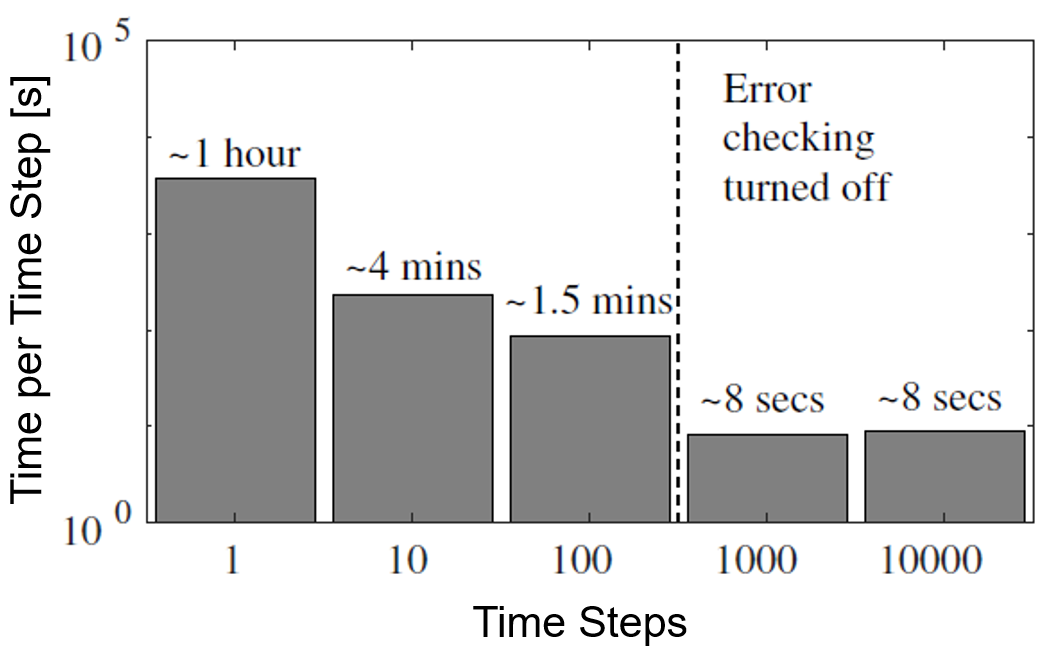
\includegraphics[width=1.03\linewidth]{Figures/Intro_Load_Bar_Graph.PNG}
    \caption{Typical evaluation time (wall clock time) for reacting flow Large Eddy Simulations. The semi-log plot illustrates an exponential decay in time per timestep, but with severe cost in initial timesteps due to chemical Jacobian construction, evaluation, and inversion.}
    \label{fig:Intro}
\end{figure}

Typically, the computational cost of the chemical source term evaluation dominates the performance metrics and creates an uneven computational load distribution in parallel applications. The difficulties occur due to the intrinsic and non-linear nature of the ODE system. Figure~\ref{fig:Intro} shows typical evaluation time for a laboratory scale jet flame \cite{Lacey_thesis}. The computational cost of solving the associated stiff ODEs scales quadratically with the number of species. Furthermore, due to the vast scale separation between the fastest and slowest chemical reaction time scales, the system of ODEs is practically always numerically stiff, requiring the use of implicit time integrators with low timestep values. \textbf{This project implements a \emph{dynamic load balancing} scheme (specifically Lend When Idle) on the low Mach number flow solver, \texttt{NGA} \cite{DESJARDINS2008,MACART2016}}. Additionally this project develops a \emph{reference mapping} paradigm to sort group cells with similar thermochemical composition, thereby evaluating their chemical source terms only when sufficiently dissimilar. The structure of the paper is as follows:
\begin{enumerate}
\item The low Mach flow solver \texttt{NGA}, its associated dependencies, and its current scheme for approximating and distributing load is introduced. Additional background is provided on numerical approaches for solution of multi-dimensional reacting flows, especially chemical source term evaluation.
\item The Lend When Idle (LeWI) scheme, an existing runtime-based, task-neutral dynamic load balancing code that distribute resources through the \texttt{MPI} protocol, is introduced and implemented with \texttt{NGA}.
\item A \emph{reference mapping scheme} based on combustion theory and multi-zone reduction models is developed and implemented.
\item The balanced \texttt{NGA} code is evaluated using two canonical turbulent jet flames. An overview of load balancing in state-of-the-art reacting flow solvers is given and directions for further future development is discussed.
\end{enumerate}

\section{Background: Existing Numerical Scheme}
\subsection{Conservation Equations and Fluid Solver}
Advanced schemes solve the coupled Navier-Stokes system using a second order MUSCL-Hancock scheme (Monotonic Upstream-Centered Scheme for Conservation Laws). This scheme was designed for solving any system of non-linear hyperbolic conservation laws. The method is employed for discretizing the governing equations, starting with a control volume $\Phi$ and flux $F$:
$$F(\Phi) \rightarrowtriangle \underbrace{\boxed{ \; \Phi \; }}_{\Delta x} \rightarrowtriangle F(\Phi + \Delta \Phi)$$ 
The conservation equations for three-dimensional, multi-component, reactive compressible flows can be written in index notation as
$$ \frac{\partial \Phi}{\partial t} + \frac{\partial F (\Phi)}{\partial x_j} + N \frac{G (\Phi)}{x_j} = \frac{\partial F_\nu (\Phi)}{\partial x_j} + S (\Phi) $$
$F_\nu$ is the diffusion flux, $S$ is the reaction term, and $G$ is the geometric shape factor \cite{Chen_thesis}. The vectors $\Phi$, $F (\Phi)$, $G (\Phi)$, $F_\nu(\Phi)$, and $S (\Phi)$ are defined as
\begin{multline*}
    \Phi = \begin{bmatrix}
    \rho Y_1 \\
    \rho Y_2 \\
    \vdots \\
    \rho Y_k \\
    \rho u \\
    E
    \end{bmatrix} \quad
    \textbf{F}(\Phi) = \begin{bmatrix}
    \rho u Y_1 \\
    \rho u Y_2 \\
    \vdots \\
    \rho u Y_k \\
    \rho {u}^2 + P \\
    (E + P) u
    \end{bmatrix} \quad
    \textbf{G}(\Phi) = \begin{bmatrix}
    \rho u Y_1 \\
    \rho u Y_2 \\
    \vdots \\
    \rho u Y_k \\
    \rho {u}^2 \\
    (E + P) u
    \end{bmatrix} \\
    \textbf{F$_\nu$}(\Phi) = \begin{bmatrix}
    \textrm{viscous terms}
    \end{bmatrix} \quad
    \textbf{S}(\Phi) = \begin{bmatrix}
    \dot{m}_1, \dot{m}_2, \dots, \dot{m}_k , 0 , 0
    \end{bmatrix}
\end{multline*}
where $N$ is the geometry factor ($N=0$, rectangular coordinate; $N=1$, cylindrical coordinate; $N=2$ spherical coordinate). $u$ is the flow velocity and $x(=r)$ is the spatial coordinate. $\rho$ represents the fluid density, $Y_k$ is the mass fraction of species $k$, $E$ is the total energy, and $P$ is the pressure of the fluid. Energy in the low Mach number limit is $E = \rho \, \textrm{e} + \cancel{\rho u^2 / 2} = \rho \, \textrm{e}$. Along with the ideal gas equation of state, these equations represent a closed system.

\subsection{Operator Splitting Technique}
Commonly, engineering flow solvers assume an operator-splitting strategy in the reacting flow implementation, enabling the decoupling of the chemistry and fluid dynamics in the solution during the calculation of the chemical source terms. Therefore, the changes in thermochemical composition $\Phi$ can be described as a stiff system of ordinary differential equations (ODEs) $\partial \Phi / \partial t = F(\Phi, t)$. A linear or non-linear system can be defined in matrix form as $\Phi \equiv \phi_{i,j} $ and $\mathbf{f}(\Phi) \equiv f_{i,j} (\Phi)$ for $ i= 1, \dots, N $, $ j= 1, \dots, N $. Parallelization is achieved with geometrical domain decomposition. The Strang splitting scheme is achieved with the spatially discretized governing equations:
$$\frac{\textrm{d} \Phi}{\textrm{d} t} = \underbracket[0.5pt]{\mathbf{T}(\Phi)}_{\textrm{transport}} + \underbracket[0.5pt]{\mathbf{S}(\Phi)}_{\textrm{chemistry}} $$
The two steps are denoted by operator $\textbf{T}^{(t)}$ (for transport) and operator $\textbf{S}^{(t)}$ (chemical source), respectively. Based on the above splitting, the solution can be evolved from its initial value $\Phi^n$ at time $t^n$, by one timestep of size $\Delta t$, to a value $\Phi^{n+1}$ at time
$t^{n+1} = t^n + \Delta t$,
$$\Phi^{n+1} = \textbf{S}^{\Delta t} \, \textbf{T}^{\Delta t} (\Phi^n)$$
The above procedure for solving the inhomogeneous system is only first-order accuracy in time. A scheme with second-order accuracy in time called Strang splitting is 
$$\Phi^{n+1} = \textbf{S}^{\Delta t / 2} \, \textbf{T}^{\Delta t} \, \textbf{S}^{\Delta t / 2} (\Phi^n)$$
where $\textbf{S}$ and $\textbf{T}$ are at least second-order accurate solution operators in time. The time derivative is approximated by finite-difference involving the current and future values. The gradient and divergence operators are approximated with linear functions involving multiple neighboring cells. Transport is relatively linear and has a highly structured Jacobian, with weak coupling between species. Chemistry is highly nonlinear and typically solved implicitly. Chemistry terms are local, so each mesh volume can be solved independently (i.e., in parallel). The chemistry and transport substeps are then:

\footnotesize
\begin{alignat*}{3}
    \frac{\textrm{d} \Phi}{\textrm{d} t} &= \mathbf{S}(\Phi^{(1)}), \qquad &&\Phi^{(1)}(x,0) = \Phi(x,t_n) \;\; & &\textrm{on} \; [t_n, t_n + \Delta t / 2] \\
    \frac{\textrm{d} \Phi}{\textrm{d} t} &= \mathbf{T}(\Phi^{(2)}), \qquad &&\Phi^{(2)}(x,0) = \Phi^{(1)}(x,\Delta t / 2) \;\; & &\textrm{on} \; [t_n, t_n + \Delta t] \\
    \frac{\textrm{d} \Phi}{\textrm{d} t} &= \mathbf{S}(\Phi^{(3)}), \qquad &&\Phi^{(3)}(x,0) = \Phi^{(2)}(x,t_n) \;\; & &\textrm{on} \; [t_n + \Delta t / 2, t_n + \Delta t]
\end{alignat*}
\normalsize
Considering the time integration of a stiff reacting system, each implicit integration step involves evaluation of the source terms by Jacobian evaluation and factorization in a Newton-Raphson scheme. A system of ODEs in chemistry is defined based on multiple chemical species $N_k$ (i.e., types of molecules) evolving through coupled reactions $d \Phi / d t = \mathbf{S} \Phi$, where $\Phi = [\phi_1, \phi_2, ... \phi_N] \in \mathbb{R}^N$ and $\mathbf{S} \in \mathbb{R}^{N \times N}$. Any time integration scheme requires the eigenvalues of $\mathbf{S}$ to lie inside the stability region of the method. The system is stiff if for the set of the eigenvalues $[\lambda_1, \lambda_2, ... \lambda_N]$ of matrix $\mathbf{S}$: $|\lambda_\textrm{max}|/|\lambda_\textrm{min}| \gg 1$. A stiff problem requires a very small timestep for stability with respect to $|\lambda_\textrm{max}|$ in conjunction with a very long time integration to see any significant change in magnitude associated to $|\lambda_\textrm{min}|$.

The system $\mathbf{S}(\Phi) = 0$ is solved first by constructing the Jacobian in 2-D $\mathbb{J} \equiv \partial S_{i,j} \, / \, \partial \phi_{i,j}$. Then the Newton-Raphson scheme computes the components of the matrix. Each iteration is defined by the linear system $\mathbb{J}(\Phi^{\, n+1} - \Phi^n) = $ -$ \mathbf{S}(\Phi^n)$ and can then be solved through direct matrix inversion sequentially,
$$ \Phi^{\, n+1} = \Phi^n - [\mathbb{J}^{-1} \cdot \mathbf{S}(\Phi^n)] \quad \textrm{.} $$
Here the Jacobian is an $N^2 \times N^2$ matrix and thus \textbf{Jacobian evaluation and factorization is the most expensive step in combustion simulations}. To solve the conservative system, the stiff source term $\textbf{S}$ is treated by the fractional-step procedure. In the first fractional step, the non-reactive flow is solved using the MUSCL-Hancock scheme from Toro \cite{Toro2009}.
\begin{equation*}
    \left.
    \begin{aligned}
        \textrm{PDE}&: \; \frac{\partial \Phi}{\partial t} + \frac{\partial F (\Phi)}{\partial x_j} + N \frac{G (\Phi)}{x_j} = \frac{\partial F_\nu (\Phi)}{\partial x_j} \\
        \textrm{IC}&: \; \Phi(x, t^n) = \Phi^n
    \end{aligned}
    \right\} \rightarrowtriangle \overline{\Phi}^{\, n+1}
\end{equation*}
\noindent \textbf{MUSCL-Hancock scheme} To numerically solve the system of equations, a second-order MUSCL-Hancock scheme (Monotonic Upstream-Centered Scheme for Conservation Laws) is used. The steps of this solver include:
\begin{enumerate}
    \item \emph{Data Reconstruction}: Cell-centered values are extrapolated into slopes between grid cells so that the fluid is represented by a piecewise-linear plane in each of the cells. The \emph{boundary extrapolated values} ($\Phi_i^L, \, \Phi_i^R, \, \Phi_j^L, \, \Phi_j^R$) are then calculated.
    \item \emph{Evolution}: Each of the four boundary extrapolated values move forward by a half timestep.
    \item \emph{Riemann Initial Value Problem}: A HLLC (Harten-Lax-van Leer-Contact) Riemann solver was implemented to calculate the fluxes in the $i$ and $j$ direction at the cell faces \cite{Toro2009}. It determines the states of nearby cells and then calculates the variable fluxes across those cells using conservation laws.
    \item \emph{Conservative Update}: The conserved variables are updated. The MUSCL-Hancock scheme is repeated for each consecutive timestep.
\end{enumerate}
\subsection{Chemical Source Term evaluation}
With this technique, chemistry can be treated as an independent stiff ODE system within each computational cell. The chemistry is solved in the second fractional step for a homogeneous system
\begin{equation*}
    \left.
    \begin{aligned}
        \textrm{ODE}&: \; \frac{d \Phi}{d t} = \textbf{S} (\Phi) \\
        \textrm{IC}&: \; \overline{\Phi}^{\, n+1}
    \end{aligned}
    \right\} \rightarrowtriangle \Phi^{\, n+1}
\end{equation*}
For the $\textbf{S}$ operator, the mass fraction of species are updated by using the \texttt{CVODE} solver \cite{SUNDIALS}. Note that the density $\rho$, momentum $\rho u$, and total energy $E$ remain constant during updating the mass fraction of all the species, after which the temperature $T$ is solved according to the definition of total energy:
$$F(T) = R_0 T / \overline{M} - u^2 / 2 - h + E / \rho = 0$$
where the equation of state $\rho = \sum \rho_i = P \overline{M} / R_0 T$ is utilized to eliminate the pressure term. The above equation can be solved numerically by using the Newton iteration method and the
updated temperature at each iteration step is
$$T^\textrm{new} = T^\textrm{old} - F(T^\textrm{old})/(R_0 / \overline{M} - c_P)$$

\subsection{Load Balancing and \texttt{NGA}}
\texttt{NGA} \cite{DESJARDINS2008,MACART2016} is a 3-D finite-difference energy-conserving low-Mach number flow solver, using derivative operators of arbitrarily high order. It is capable of solving the variable-density Navier-Stokes equations on structured meshes using a fractional-step method. Spatial discretization errors are reduced using local $(n-1)$-th order Lagrange polynomial interpolation to achieve $n$-order accurate viscous terms. The code utilizes detailed temperature- and composition-dependent transport and thermodynamic properties, detailed chemical kinetics, and an ideal gas equation of state. \texttt{NGA} was written for massively parallel large-eddy simulation (LES) and direct numerical simulation (DNS) of both premixed and non-premixed reacting turbulent flows. It is parallelized using a hybrid \texttt{MPI}/\texttt{OpenMP} approach and is highly scalable. \texttt{NGA} uses an operator splitting technique to decouple the conservation equations and chemical source term calculations.

\begin{figure}[h!]
    \centering
    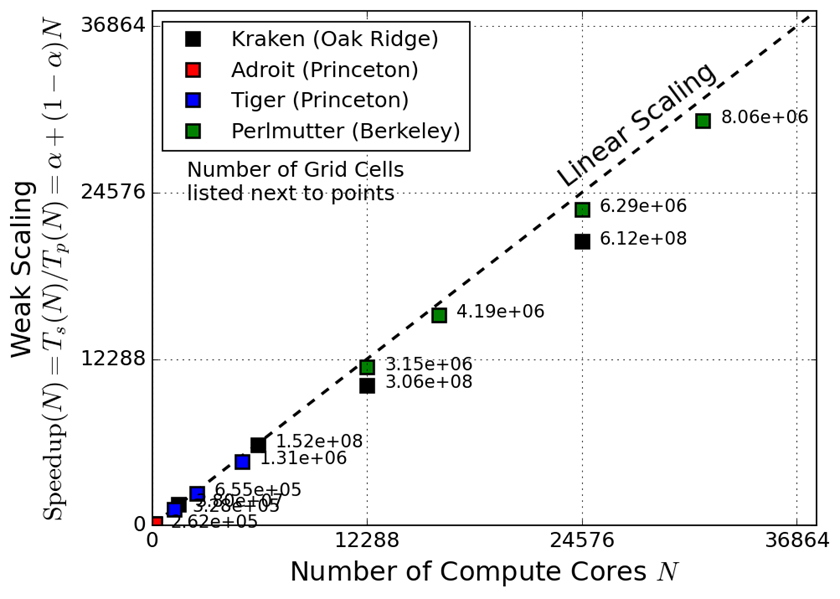
\includegraphics[width=1.03\linewidth]{Figures/NGA_scaling.PNG}
    \caption{\texttt{NGA} exhibits excellent scale-up characteristics on various high performance architectures. Scaling studies were conducted by increasing the grid resolution and number of processors while maintaining $\sim 256$ cells per core. The largest run so far has consisted of over 1.6 billion cells, and almost 50,000 compute cores.}
    \label{fig:Scaleup2}
\end{figure}

\texttt{NGA} then uses \texttt{SUNDIALS} \cite{SUNDIALS} (SUite of Nonlinear and DIfferential/ALgebraic equation Solvers) \texttt{CVODE} (unsteady solver) for solving stiff systems of initial value ODEs for detailed chemistry (chemical Jacobian construction, inversion, and Newton iteration). Load balancing is not handled internally by the \texttt{SUNDIALS} integrators but rather is the responsibility of the application developer. As a result of the highly non-linear characteristics of chemical kinetics, a large variation in the convergence rates of the ODE integrator may occur, leading to a high load imbalance across multiprocessor configurations. However, the independent nature of chemistry ODE systems leads to a problem that can be parallelized easily (embarrassingly parallel) during the flow solution. The presented LeWI model takes advantage of this feature and balances the chemistry load across available resources.

Because the ODEs are uncoupled across the domain, there is considerable freedom in staging their integration. In multi-threaded CPU-based implementations, the total work to integrate all the cells in the domain can be distributed arbitrarily across the available threads with no race or synchronization concerns. \texttt{NGA} currently uses a rudimentary load balancing scheme by approximating the work for each cell ahead of time by tracking the work required to integrate the previous timestep. Thus, it is in the earliest timesteps that more robust load balancing scheme could provide considerable speed-up.

\section{Implementation}
\subsection{Systems Component: \\Dynamic Load Balancing}
Lend When Idle \cite{LeWI_ICPP09,GARCIA2014,DLB_OpenMP_SMPS} (LeWI) is a novel \emph{work stealing} \cite{Work_Stealing} algorithm that distributes resources equally among \texttt{MPI} processes in a node while they are doing computation, and re-assigns resources of \texttt{MPI} processes while they are blocked in communication calls. One of its main properties is that the load balancing is task neutral, done dynamically at runtime without analyzing nor modifying the application previously. This dynamism allows LeWI to react to different sources of imbalance: algorithm, data, hardware architecture, and resource availability.

Figure~\ref{fig:Diagram_LeWI} shows an example of how the algorithm works. The application is running in a node with 4 CPUs. It starts two \texttt{MPI} processes in the same node and each \texttt{MPI} process spawns 2 \texttt{OpenMP} threads. \texttt{MPI} process 1 gets into the blocking call and will lend its two \texttt{OpenMP} threads to the \texttt{MPI} process 2. The second \texttt{MPI} process will use the newly acquired CPUs as fast as the programming model allows it. When the \texttt{MPI} process 1 gets out of the blocking call it retrieves its CPUs from the \texttt{MPI} process 2 and the execution continues with an equal CPU partition until another blocking call is met.

The LeWI scheme has previously been implemented with both \texttt{OpenMP} and \texttt{SMPSuperscalar} protocols at the inner layer of parallelism \cite{DLB_OpenMP_SMPS}. Because \texttt{NGA} is parallelized in a hybrid \texttt{MPI}/\texttt{OpenMP} approach, the following description will only consider \texttt{OpenMP}. \texttt{OpenMP} is limited by the fork-join model and can only change the number of threads outside a parallel region (e.g., ``DO'' loop). This means that when an \texttt{MPI} process lends its CPUs, the \texttt{MPI} process that wants to use them is not able to do so until reaching a new parallel region. This limitation makes the performance of the algorithm highly dependent on the number of parallel regions that the application presents between \texttt{MPI} blocking calls. 

The LeWI module is used in hybrid \texttt{MPI}/\texttt{OpenMP} applications to dynamically and transparently change the process number of threads and their CPU affinity. LeWI mode must be enabled before using the environment variable \texttt{DLB\_ARGS} with the value \texttt{--lewi}, and optionally \texttt{--lewi-keep-one-cpu}. Then, place calls to \texttt{DLB\_Borrow()} before parallel regions with a high computational load, or at least those near \texttt{MPI} blocking calls. LeWI cannot manage the CPU pinning of each thread and so each \texttt{MPI} rank is run without exclusive CPU binding:

{\tt \small
\begin{verbatim}
$ mpicc -fopenmp opt.c -o opt -I"$DLB_PREFIX/include"\
        -L"$DLB_PREFIX/lib" -ldlb_mpi -Wl,\
        -rpath,"$DLB_PREFIX/lib"
$ export DLB_ARGS="--lewi"
$ mpirun -n 2 --bind-to none ./opt
\end{verbatim}
}
\noindent
where \texttt{opt} is the \texttt{NGA} \texttt{makefile}. By intercepting \texttt{MPI} calls, LeWI is able to detect when the process reaches a state where the worker threads are idle, then it may temporarily yield the process assigned CPUs to another process that would benefit from them.

\begin{figure}[h!]
    \centering
    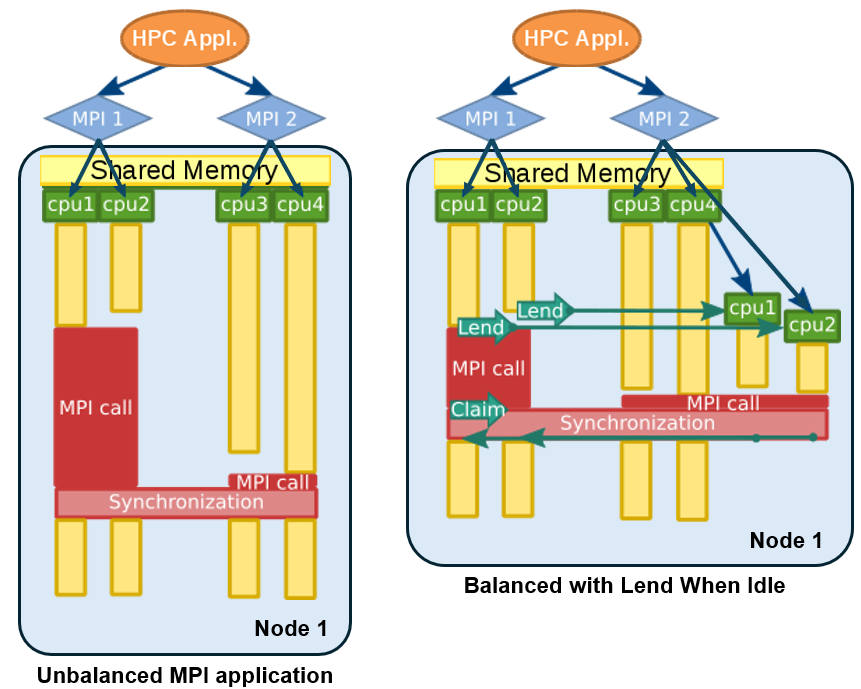
\includegraphics[width=1.03\linewidth]{Figures/LeWI_Diagram.PNG}
    \caption{Diagram of \texttt{MPI} thread execution with and without LeWI protocol. Figure adapted from \cite{LeWI_ICPP09}.}
    \label{fig:Diagram_LeWI}
\end{figure}

In using the \texttt{OpenMP} protocol, both actions (lend and retrieve) are restricted in execution one when entering a new parallel region. Thus while retrieving CPUs the application can run with more threads than CPUs available. If there are more than two \texttt{MPI} processes running in the same node the algorithm must decide to which \texttt{MPI} process (of the ones still running) lends the idle CPUs. Each time a idle CPU is waiting to be assigned the algorithm calculates a load factor for each \texttt{MPI} process. This load factor is obtained by dividing the computational load of the \texttt{MPI} process by the number of threads it has assigned. The idle CPU will be assigned to the \texttt{MPI} process with the higher load factor. For iterative applications, the computational load of each \texttt{MPI} process will correspond to the time accumulated since the beginning of the application.

In the context of reacting flow simulation, the reaction source term for an individual cell can be computed independently from all other cells, through operator splitting as described in previous sections. However, due to the non-linear nature of chemistry, the floating point operations required to evaluate source terms can vary significantly from cell to cell. The computational geometry is decomposed using available domain decomposition algorithms. However, dividing the domain geometrically into blocks of close to equal cell count may lead to chemical imbalance due to the different convergence rates of chemistry ODE problems within processes. Hence, it is beneficial to send some of the chemical problems from the overloaded processors (senders) to the less occupied processors (receivers) for more uniform load balancing. Once the chemistry calculation has been completed, the roles interchange once the updated chemical solutions are sent back to where they physically belong, as source terms in the conservation equations.

\subsection{Programming Languages Component: \\Reference Mapping scheme}
\noindent The timestep value and hence the total number of floating-point operations during the integration depends on the initial thermochemical composition. Parallelization is achieved with geometrical domain decomposition, leading to explicit chemistry load imbalance due to spatially and temporally varying values. A simple reference mapping feature allows a further reduction in computational cost. This approach groups cells sharing similar thermochemical composition values together and solving the chemistry only once for this group \cite{DLBFoam_1}. Such a mapping approach is intended to be used for regions with low reactivity, (e.g., where no fuel is present or in low-temperature regions far upstream and downstream of the flame, where few chemical reactions are occurring), similar to multi-zone reduction models \cite{Zonal}. \textbf{The reference mapping acts as a filter for load balancing, where the reaction rates of cells satisfying a user-given criteria are copied from a reference cell solution.} At a given time instance, a reference cell is picked and the chemistry source term of that cell is solved and copied to other reference cells. The criteria used for identifying the reference cells is: $Z_i < Z_\textrm{tol}$, $|T_i - T_\textrm{ref} | < T_\textrm{tol}$, where $Z_i$ and $T_i$ are mixture fraction (the mass fraction of fuel in a fuel/oxidizer stream, a conserved scalar with no source term) and temperature of $i$-th cell, respectively, $T_\textrm{ref}$ denotes the temperature of the chosen reference cell and $Z_\textrm{tol}$ and $Z_\textrm{tol}$ are the user-defined tolerance values, specified in the \texttt{input} and \texttt{config} files.

The reference mapping implemented is applied to each process separately. As long as conservative tolerances are used, the introduced error is rather small and does not affect the global characteristics of the reactive simulation. Figure~\ref{fig:RefMap} illustrates the partitioning of cells, where the gray cells indicate regions of low reactivity and are not evaluated, but rather mapped to a similarly low reactivity reference cell. The error is likely negligible compared to typical uncertainties found in various combustion models. The reference mapping model improves the balancing performance significantly by further reducing the load of the more idle processes and increasing their potential to receive more load from the busier processes.

\begin{figure}[h!]
    \centering
    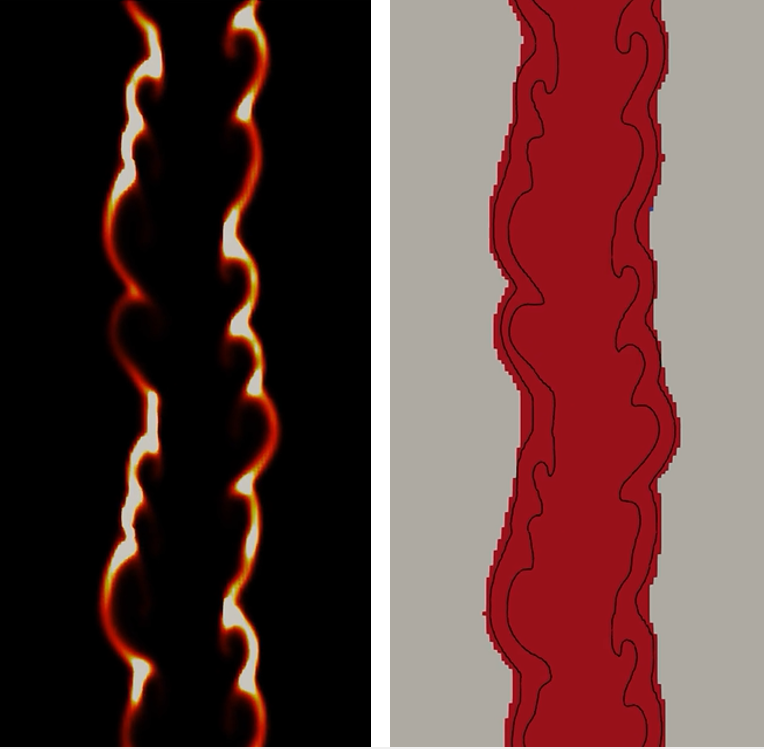
\includegraphics[width=\linewidth]{Figures/Ref_Map.PNG}
    \caption{Visualization of the reference mapping implemented in Sandia Flame D. (\textbf{left}) Colored by heat release rate, (\textbf{right}) \textcolor{red}{\textbf{red}} cells are those with full chemical Jacobian evaluation, \textcolor{gray}{\textbf{gray}} cells are those where a non-reacting reference cell is copied. $Z_\textrm{tol} = 10^{-2}$ and $T_\textrm{tol} = 1$ [K].}
    \label{fig:RefMap}
\end{figure}

\section{Evaluation}
\subsection{Benchmarks}
Runtime performance is evaluated by comparing to simulations of hydrogen-air and methane-air jet flames. These configurations were initially experiments from the turbulent non-premixed flames (TNF) workshop \url{https://tnfworkshop.org/} and are representative of laboratory-scale problems in the combustion science field.  These experiments were replicated using Large Eddy Simulation in \texttt{NGA} without load balancing and published by Lacey et al. \cite{LACEY2021,Lacey_thesis}. The experimental data agrees strongly with the simulation, validating the \texttt{NGA} modeling paradigm within acceptable accuracy for these cases. The two jet flames are shown qualitatively in Figure~\ref{fig:Benchmarks}.
\\ \\  \noindent
\textbf{Configuration I: Hydrogen Jet Flame}
The first configuration is a turbulent non-premixed hydrogen jet flame with a Reynolds number of 10,000 \cite{TNF,BARLOW1994,BARLOW1996}. Only pure hydrogen, undiluted by helium, is considered in this work. The flame was simulated in cylindrical coordinates using a stretched grid with $256 \times 144 \times 64$ grid points along the axial, radial, and circumferential directions, respectively. A uniform inlet velocity profile was imposed for the coflow, and the central jet inflow velocity profile was generated from a separate simulation of fully-developed turbulent pipe flow. The chemical mechanism for hydrogen combustion \cite{Li2004} consists of 9 species and 21 reactions. For this flame, statistics were computed using a constant Smagorinsky constant of 0.12 and a constant turbulent Schmidt number of 0.7. However, timings are shown with the dynamic models for comparison with the other flame configuration.
\begin{figure}[h!]
    \centering
    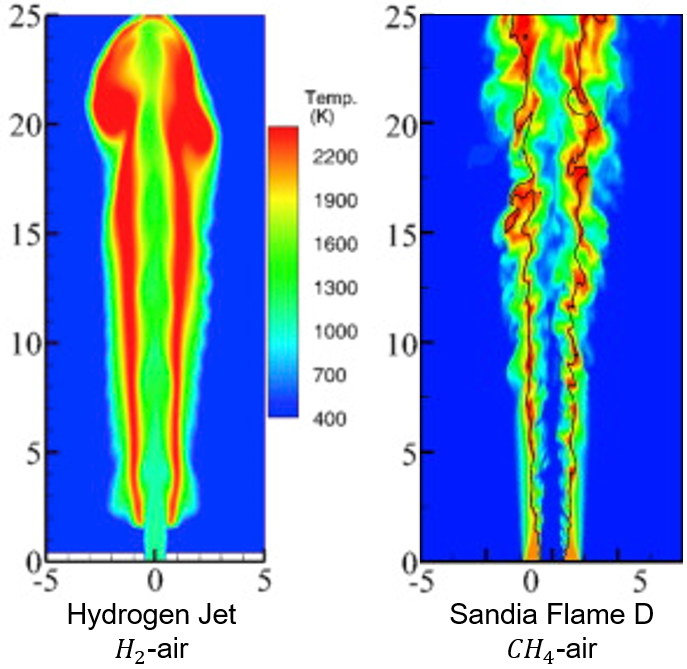
\includegraphics[width=1.03\linewidth]{Figures/Benchmarks.PNG}
    \caption{Hydrogen Jet and Sandia Flame D benchmark test cases. Flames are axially symmetric. Spatial numbering represents normalization by the jet diameter: radial ($r/D$) and axial ($x/D$). Colored by temperature.}
    \label{fig:Benchmarks}
\end{figure}
\\ \\ \noindent
\textbf{Configuration II: Sandia Flame D}
The second configuration is Sandia Flame D, a turbulent piloted partially premixed methane/air jet flame with a Reynolds number of 22,400 \cite{TNF,BARLOW1998}. The flame was simulated
in cylindrical coordinates using a stretched grid with $256 \times 144 \times 64$ grid points along the axial, radial, and circumferential directions, respectively. Uniform inlet velocity profiles were imposed for the coflow and pilot, and the central jet inflow velocity profile was generated from a separate simulation of fully-developed turbulent pipe flow. The mechanism for methane combustion, \texttt{GRI-3.0} \cite{gri30}, consists of 35 species with the nitrogen chemistry removed.

\subsection{Lend When Idle Results}
To achieve statistical convergence, the simulations were run for 30 characteristic ``flame time scales'' in accordance with the pseudo-Central Limit Theorem. The chemical timescale $\tau_C$ is the laminar flame thickness divided by the laminar burning velocity. For hydrogen, $\tau_C = 0.204$ [msec] and for methane $\tau_C = 1.18$ [msec]. Thus the simulations were run to completion $30 \, \Delta t \cdot \tau_C$. Figures~\ref{fig:ResultH2} and \ref{fig:ResultD} show the wall clock time per simulation timestep for the Hydrogen Jet and Sandia Flame D, respectively, in a semi-log bar graph. Here, the comparison of ``time per timestep'' for the balanced and unbalanced simulations serves as an indicator for load balancing. Each simulation timestep will be shorter with computational resources saturated (improved parallel efficiency), all else constant.

\begin{figure}[h!]
    \centering
    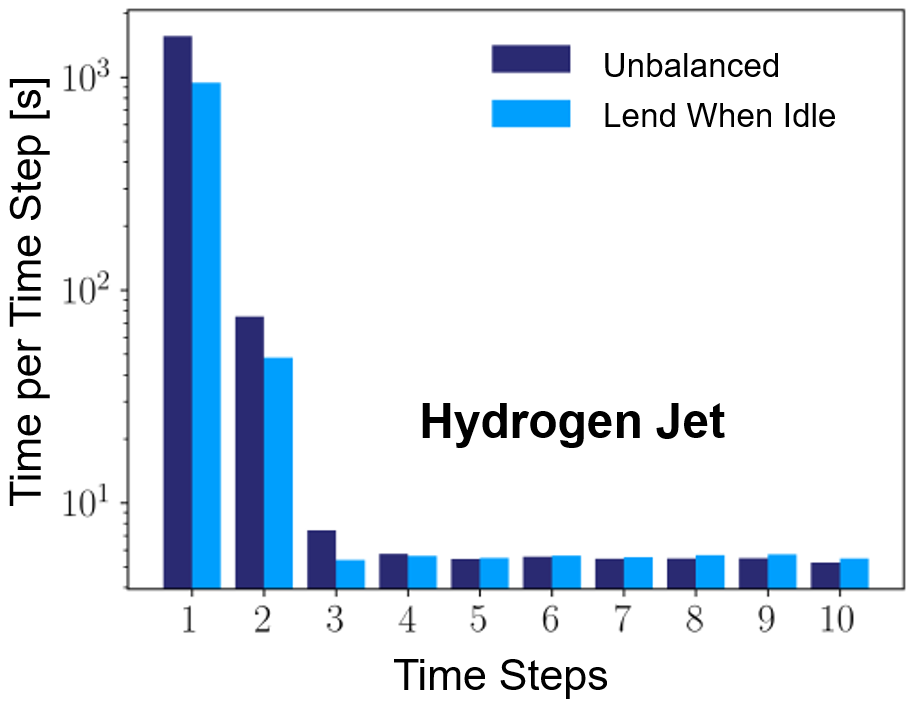
\includegraphics[width=1.03\linewidth]{Figures/H2_Results.PNG}
    \caption{Wall clock time per timestep in the Hydrogen Jet simulation for both the balanced and unbalanced cases. For equal problem size, time per timestep is an indicator of parallel efficiency.}
    \label{fig:ResultH2}
\end{figure}
\begin{figure}[h!]
    \centering
    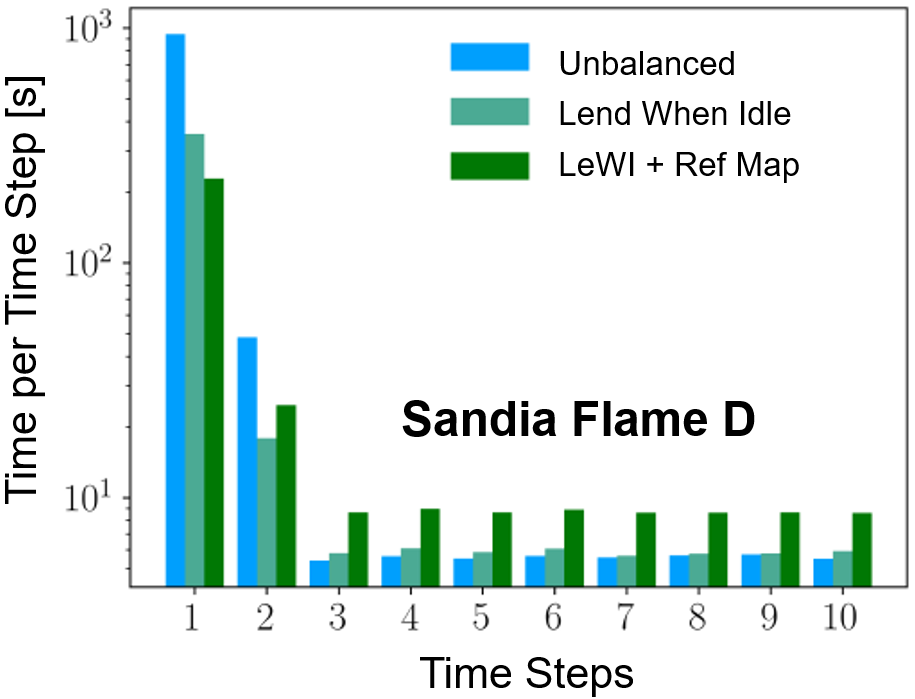
\includegraphics[width=1.03\linewidth]{Figures/Sandia_D_Results.PNG}
    \caption{Wall clock time per timestep in the Sandia Flame D simulation for both the balanced and unbalanced cases, as well as balanced with reference mapping. For equal problem size, time per timestep is an indicator of parallel efficiency.}
    \label{fig:ResultD}
\end{figure}

It can be seen that, as discussed in previous sections, the first timesteps are extremely costly, taking nearly an hour, due to the highly non-linear initialization of flow and chemical systems. The unbalanced \texttt{NGA} solver then estimates the load for each cell using what was required to integrate the previous timestep. For these test cases, the simulation quickly plateaus to only a few seconds per timestep by the 3rd or 4th timestep. It can be seen that Lend When Idle provides a modest improvement between 10\% and 30\% for the earliest timesteps. In later timesteps, the speed is comparable and slightly slower than the unbalanced version. This is likely due to the additional I/O bottleneck overhead associated with \texttt{MPI} calls that may be unnecessary for already fast calculations. A future implementation feature may be to ``turn off'' Lend When Idle after certain speed plateau criteria are met. Nonetheless, the speedup in the initial timesteps significantly reduces the cumulative simulation time.

\subsection{Reference Mapping Results}
The reference mapping model should improve the balancing performance modestly by further reducing the load of the more idle processes and increasing their potential to receive more load from the busier processes. Implemented only for Sandia Flame D in Figure~\ref{fig:ResultD}, the scheme provides a further improvement beyond load balancing alone for the initial timesteps. However, past the speed plateau, the scheme slows down iterative timesteps by a factor of 2. This is likely because the scheme is implemented as a looping function through all cells in the domain, which as the flame reaches steady-state, becomes significant in the overall evaluation. This feature too may be worth ``turning off'' beyond the plateau. 

Lend When Idle is purely a manipulation of Message Passing Interface protocol to improve parallel efficiency and makes no assumptions or corrections to the flow physics and chemistry. However, reference mapping seeks to mitigate load imbalance using a custom decomposition with a prior knowledge on the spatial activity of chemical kinetics, which will introduce errors. As long as properly strict tolerances are used (chemical reactions are highly non-linear based in an Arrhenius law), the introduced error should be rather small and not affect the global characteristics of the reactive simulation. 

Figure~\ref{fig:Error} quantifies the error introduced by the reference mapping model. The figure shows the $L_2$ norm of the error of the volume integral of the heat release rate $\int_V \dot{\omega} \,\, dV$ over all time instances relative to the results obtained with the standard chemistry model. The results are obtained from the Sandia Flame D case with mixture fraction tolerances $Z_\mathrm{tol} = 10^{-6}$-$10^{-2}$ and $T_\mathrm{tol} = 1$ [K] fixed. The norm of error is shown for simulations of increasing total number of cells $N$. When the load balancing algorithm is used without mapping, identical results to the standard model are obtained for all process counts as expected. When the reference mapping is used, overall errors are small, approaching machine precision and scale as $\mathcal{O}(\log(N))$. Spikes in error corresponding to non-powers of 2 are a result of the number of processors per node on the computer hardware. Initially a large deviation around 10\% is observed for $Z_\mathrm{tol} = 10^{-2}$. With tighter tolerances, this error drops to below 2\%.

\begin{figure}[h!]
    \centering
    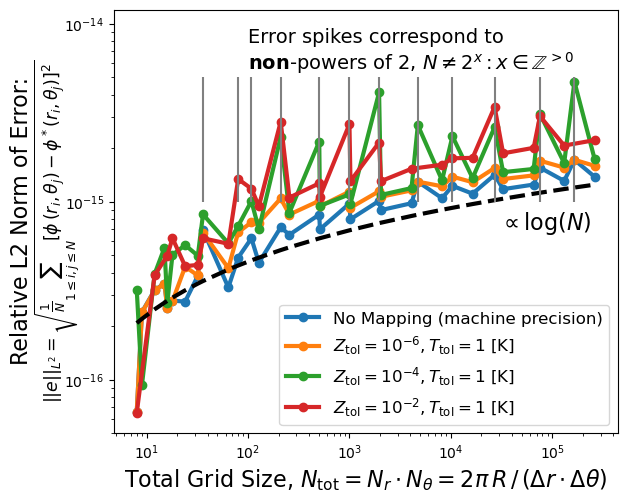
\includegraphics[width=1.03\linewidth]{Figures/Ref_Error.PNG}
    \caption{$L_2$ norm of the error of the volume integral of the heat release rate $\int_V \dot{\omega} \,\, dV$ over all time instances relative to the results obtained with the standard chemistry model for increasing problem (total grid) size.}
    \label{fig:Error}
\end{figure}

\section{Related Work: Load Balancing in other \\reacting flow solvers}
Most advanced reacting flow solvers like \texttt{Pele} \cite{PeleC,PeleMP} and \texttt{OpenFoam} \cite{DLBFoam_1,DLBFoam_2} are built on the \texttt{AMReX} structure \cite{AMReX}. \texttt{AMReX} is a publicly available software framework designed for building massively parallel block-structured adaptive mesh refinement (AMR) applications. \texttt{AMReX} provides a very general approach for decomposition of the computational domain into individual logically rectangular grids, and how to distribute those grids to \texttt{MPI} ranks. The load balancing process combines grid creation (and re-creation when regridding) and distribution of grids to \texttt{MPI} ranks.

For single-level calculations, \texttt{AMReX} provides the flexibility to have different size grids, more than one grid per \texttt{MPI} rank, and different strategies for distributing the grids to \texttt{MPI} ranks. For multi-level calculations, the same principles for load balancing apply as in single-level calculations, but there is additional complexity in how to tag cells for refinement. The process of load balancing is typically independent of the process of grid creation; the inputs to load balancing are a given set of grids with a set of weights assigned to each grid.

Single-level load balancing algorithms are sequentially applied to each AMR level independently, and the resulting distributions are mapped onto the ranks taking into account the weights already assigned to them (assign heaviest set of grids to the least loaded rank). Note that the load of each process is measured by how much memory has already been allocated, not how much memory will be allocated. Distribution options supported by \texttt{AMReX} include the following (the default is SFC):
\begin{itemize}
\setlength\itemsep{0.01em}
    \item \textbf{Knapsack}: the default weight of a grid in the knapsack algorithm is the number of grid cells, but \texttt{AMReX} supports the option to pass an array of weights--one per grid--or alternatively to pass in a MultiFab of weights per cell which is used to compute the weight per grid.
    \item \textbf{SFC}: enumerate grids with a space-filling Z-morton curve, then partition the resulting ordering across ranks in a way that balances the load.
    \item \textbf{Round-robin}: sort grids and assign them to ranks in round-robin fashion--specifically FAB $i$ is owned by CPU $i \in N$ where $N$ is the total number of \texttt{MPI} ranks.
\end{itemize}

\section{Future Work}
Apart from the optimization of the ODE solver algorithms themselves, several modeling strategies have been proposed to reduce the high computational requirements associated with reacting flows. In particular certain strategies are formulated in a ``processor-based'' approach, being still prone to yield computational load imbalance across available resources.

\begin{figure}[h!]
    \centering
    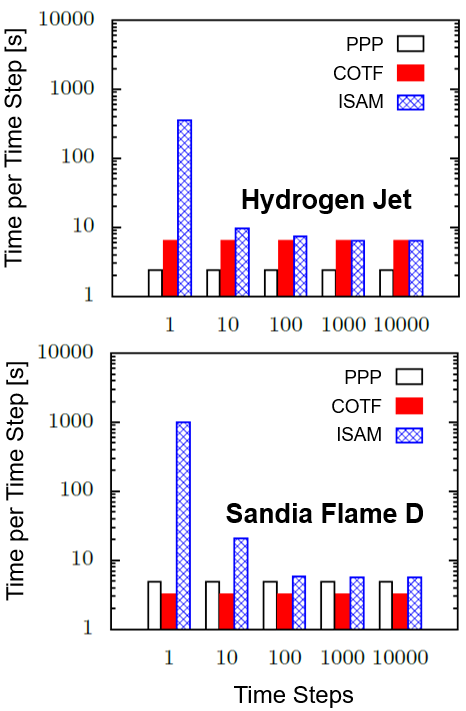
\includegraphics[width=\linewidth]{Figures/ISAT.PNG}
    \caption{Baseline performance of In-Situ Adaptive Manifold (ISAM) modeling and Convolution-on-the-Fly (COTF) compared to solutions without any optimizations (pre-computed, pre-convoluted, and pre-tabulated, PPP) for the Hydrogen Jet and Sandia Flame D. Reproduced from \cite{LACEY2021}.}
    \label{fig:ISAT}
\end{figure}

Schemes like In-Situ Adapative Manifold (ISAM) modeling and Convolution-on-the-Fly (COTF) developed by Lacey et al. \cite{LACEY2021} are based on binary-tree search. Thus are costly in the early timesteps as the tree of thermochemical state solutions is built. The cost sharply declines over the first ten timesteps and rapidly reaches a plateau for both test cases, shown in Figure~\ref{fig:ISAT}. Thus it may be the case that a load balancing scheme, as implemented in this work, could provide a beneficial speed improvement in the early timesteps.

\section{Conclusion}
Computational load imbalance across large-scale parallel computing architectures can significantly slow simulations of chemically-reacting fluid flows, like combustion. The exponential nature of reaction kinetics makes evaluation of chemical sources terms highly sensitive to local conditions, making prediction and balancing of computational load difficult. This project implemented a dynamic load balancing scheme (Lend When Idle) on a massively parallel low Mach number flow solver \texttt{NGA}. Additionally this project developed a reference mapping paradigm to sort group cells with similar thermochemical composition, thereby evaluating their chemical source terms only when sufficiently dissimilar. A modest speed-up is demonstrated for Large Eddy Simulations of two turbulent jet flames, particularly for early simulation timesteps, where computational load is most difficult to predict. These jet flames are characteristic of laboratory-scale problems. It is believed this load balancing scheme will pair well with several processor-based modeling strategies to reduce the high computational requirements associated with reacting flows.

\section{Acknowledgments}
This material is based upon work supported by the U.S. Department of Energy, Office of Science, Office of Advanced Scientific Computing Research, Department of Energy Computational Science Graduate Fellowship under Award Number DE-SC0024386.

The work presented was substantially performed using the Princeton Research Computing resources at Princeton University which is consortium of groups led by the Princeton Institute for Computational Science and Engineering (PICSciE) and Office of Information Technology's Research Computing. 

This research used resources of the National Energy Research Scientific Computing Center (NERSC) at Lawrence Berkeley National Laboratory (LBL), a Department of Energy Office of Science User Facility using NERSC award DDR-ERCAP0026889 (project m1266).

{\footnotesize \bibliographystyle{acm}
\bibliography{references}}


\theendnotes
\noindent
The core code libraries for the results presented are available at the following repository, including instructions for running and compiling.
\\ \\ \noindent
Github: \url{https://github.com/mw6136/NGA_LeWI}
\appendix


\end{document}







